\newpage
%%%%%%%%%%%%%%%%%%%%%%%%%%%%%%%%%%%%%%%%%%%%%%%
%%%%%%%%%%%%%%%%%%%%%%%%%%%%%%%%%%%%%%%%%%%%%%%
%%%%%%%%%%%%%%%%%%%%%%%%%%%%%%%%%%%%%%%%%%%%%%%
\setcounter{section}{2}\section{日本が狙う科学的課題}
\label{c06.s3}

この節では日本が狙う宇宙磁場研究をまとめる。まず日本の戦略の方針を決めるために検討した日本の独自性と優位性をまとめる。続いて日本のサイエンス事例を紹介していく。

%%%%%%%%%%%%%%%%%%%%%%%%%%%%%%%%%%%%%%%%%%%%%%%
%%%%%%%%%%%%%%%%%%%%%%%%%%%%%%%%%%%%%%%%%%%%%%%
\subsection{はじめに}
\label{c06.s3.ss1}

\paragraph{宇宙磁場研究の本質:多様性と普遍性}

ここまでの紹介で、磁場は宇宙の豊かな構造を形作っていると分かるだろう。そのような多様性が、宇宙磁場研究の魅力である。その一方で、磁場はどこへいっても磁場である。磁場の整列、乱流、宇宙線など、磁場の関わる問題には天体によらない普遍性がある。そのような普遍性もまた、宇宙磁場研究の魅力である。これらの多様性と普遍性を持つ磁場を探求するのに、特定の天体だけに注目するのはあまり適切ではない。宇宙磁場のどれかを観測的に調べるときに、前景・背景の磁場を理解していないとデータの解釈を誤る恐れがあることも注意しなければならない。前景・背景を幅広く注視することは、宇宙再電離21cm線の観測、宇宙背景放射偏光の観測、そして最高エネルギー宇宙線の観測など、磁場そのものではないが現代の挑戦的な科学的課題においても重要なことである。

\paragraph{国際SKA宇宙磁場科学検討班の戦略}

事実、国際SKA宇宙磁場科学検討班は、特定の天体の磁場研究に特化することを目指していない。代わりに、高密度なRMグリッドを用いた磁場研究という方法論を、最も優先度の高いサイエンスに選んだ。RM観測点が平方度あたり現在の1個から100-1000個へと増えれば(図\ref{c06.s2.ss1.f1})、磁場の空間構造の革新的な研究が可能となる。数の増加は赤方偏移空間にも十分な数の偏波源を与えるため、時間軸方向の変化もかつてないほど詳細に探ることを可能にする。ゆえに偏波源数を増やすため、広視野で高感度かつ高分解能の観測が求められる。既存の観測施設の延長では達成不可能であり、SKAのような大望遠鏡が不可欠である。

\paragraph{日本SKA宇宙磁場科学検討班の戦略}

国際的な戦略を考慮したうえで、日本も特定の天体の磁場研究に特化しない。代わりに日本の独自性として、偏波解消とファラデートモグラフィーに注目する。偏波解消やファラデートモグラフィーは、多くの観測対象でこれまでに知り得なかった奥行きの磁場分布の知見をもたらすので、前景・背景の磁場を包括的に理解していくという方針に合致する。その達成のためには、高分解能で高感度かつ超広帯域の観測が求められる。これらの達成も既存の観測施設の延長では不可能であり、SKAのような大望遠鏡が不可欠である。

\paragraph{日本の優位性}

日本の優位性として、特定の天体の磁場研究だけに特化しないという方針に見合うだけの、様々な天体の磁場研究者がいる点が挙げられる。その研究者らの意見交換は磁場の多様性と普遍性を見誤らないために役立っている。日本SKA宇宙磁場科学検討班でも、その科学検討において特定の天体の磁場に狙いを絞ることはせず、同班が主催している日本SKAサイエンス会議「宇宙磁場」においても、太陽から宇宙論までの磁場を討論する研究会としてきた。

\paragraph{日本が狙う科学的課題}

科学要求を満たす大望遠鏡としてSKAを建設し、そして解釈の鍵となる様々な天体の磁場の知見を持って臨めば、従来の2次元的な磁場研究は一挙に4次元的な磁場研究へと飛躍するだろう。これこそが宇宙磁場研究の次の時代のブレイクスルーである。そこで
\begin{center}
{\bf \Large 「偏波解消とトモグラフィーで紐解く4次元宇宙磁場」}
\end{center}
と題し、日本が狙う10の科学的課題を紹介する。各小節は基本的に独立して読み進めることができるように編集したが、偏波解消とトモグラフィーをキーワードに、前景や背景のことまで念頭に入れながら読み進めて頂くことを勧める。

\paragraph{日本が参画すべき開発}

上記のブレイクスルー達成のために必要な開発課題の一つは、広帯域な電波・偏波強度スペクトルデータをどのように処理するかである。SKA時代の偏波解消とトモグラフィーのためのデータ処理の方法論は、基礎理論的にも技術的にもまだ成熟しているとはいえず、日本の科学的課題を達成する水準に達しているとは言えない。ゆえに日本の科学的課題を達成するためには、大規模に組織的に日本がデータ処理のソフトウェア(あるいは専用ハードウェア)開発に責任を負うことが重要である。そこで日本ですでに進めているトモグラフィーの諸問題の改善を、日本が狙う11個目の科学的課題としてまとめた。

\paragraph{日本の様々な観測計画との強力}

加えて、日本では様々な波長と方法を用いた多岐にわたる分野の研究プロジェクトがある。それらの中には、SKA宇宙磁場研究と潜在的に協力が見込まれるものもある。そこで、さらなるシナジーを求めてと題して、多分野の関連する研究との協力も日本が狙う科学的課題の1つとしてまとめた。

\paragraph{日本の宇宙磁場研究の科学・技術要求の要約}

サイエンスで前提としている科学・技術要求は共通する所が多いので、ここでまとめる。特記のない限り、以下のような科学・技術要求となる。
\begin{itemize}
\item {\bf 核となる周波数帯域は300 MHz -- 3 GHz}\\
偏波解消とファラデートモグラフィーに注目するために最低限必要な帯域である。サーベイの効率化と電力削減のために、広帯域フィード1台で行うのが望ましい。または視野の広い密開口アンテナやフェイズドアレイフィードを採用されたい。これ以上の高周波データも偏波解消や宇宙線スペクトルの研究のためにぜひ取得したいが、視野が著しく狭くなるため、サーベイではなくフォローアップ的なスポット観測が現実的かもしれない。連続波と輝線の同時観測をズームバンド技術などによって実現すればサーベイ時間を有効活用できる。周波数非等分サンプラーは波長2乗空間でデータを均等収集でき、トモグラフィーには有効と考えられる。ただしその場合、他の観測と相乗りするならば折衝が必要となるだろう。
\item {\bf 5年間の主要科学計画(KSP)、全天1 $\mu$Jy観測や400平方度0.1 $\mu$Jy観測}\\
5年間運用のために、低電力・高信頼性の受信機や冷却系、アンテナの管理運営能力が必要である。5年(43800時間)のうち、KSPの連続波と輝線の観測を25 \%づつ、公募観測を10 \%、そしてダウンタイムを40 \% (VLAがJVLAへと拡張された2010年以降の4年平均)とすると、約10000時間、連続線観測に割り当てが可能である。一例として、南北銀極の計400平方度を0.1 $\mu$Jyにて観測する場合(たとえば図\ref{c06.s2.ss3.f2})、標準フィードの視野0.5平方度あたりSKA2で必要な予想積分時間は1時間弱なので、計800時間程度で達成する。これに較正やオーバーヘッドを加えても、割り当ての時間内で十分達成可能だろう。同様の時間で全天40000平方度を1 $\mu$Jy感度にて走査もできるだろう。なお、もしパルサーとの相乗り観測を想定するなら、ポインティングあたりの積分時間の調節が必要になる。いずれにせよ、このような長時間観測はKSPでなければ認められない。KSPで論文筆頭著者となるためには、メンバー国参加が必須である。
\item {\bf 分解能は1 GHzで$0.1''$、対応する最大基線長は1000 kmクラス}\\
SKA1では100 kmクラスの最大基線長により1 GHzで$1''$の分解能がある。SKA2でも感度の紛れ込み限界(confusion limit)を避けるため、そして狙うサイエンスのため、さらなる高分解能は不可欠であり、ゆえにこのような巨大な望遠鏡の建設を求める。SKA1はリアルタイム相関処理を行うので、もしそのままSKA2へと延長するならば、リアルタイム相関処理に必要なデータ転送速度幅は10 Gbps以上と見込まれる。
\item {\bf 最大検出角度スケールは3 GHzで$1^\circ$程度}\\
MIDアンテナ群の最小基線長が計画通り20 m程度であるならば、最大検出角度スケールは1.5 GHzで$0.5'$程度である。星間や銀河団の一部サイエンスを除けば、十分な最大検出角度スケールだろう。星間や銀河団の広がった放射のスペクトルの研究では、3 GHzで$1^\circ$程度の最大検出角度スケールを確保し、ミッシングフラックスの影響を極力減らしたい。そのためには大型単一鏡ないし基線長が数~mの小型干渉計が必要である。これはSKA2にも収まらない日本独自の構想である。
\item {\bf トモグラフィーの科学データ処理}\\
SKA2ではおそらく1億以上の背景偏波源を探知する。これは人の手で処理できる数ではない。そこでデータパイプライン自動処理が不可欠である。ゆえにどのように自動化するかという検討とそれを実現するソフトウェアの開発が必要である。なおSKA1では探知した全ての偏波源についてファラデースペクトル情報を取得する見込みであり、計算機リソースにも織り込まれている。
\end{itemize}

%%%%%%%%%%%%%%%%%%%%%%%%%%%%%%%%%%%%%%%%%%%%%%%
%%%%%%%%%%%%%%%%%%%%%%%%%%%%%%%%%%%%%%%%%%%%%%%
\subsection{銀河磁場の起源と進化}
\label{c06.s3.ss2}

\paragraph{銀河磁場の物理}

天の川銀河に現存する大局磁場の維持生成機構を明らかにすることは、銀河磁場の起源と進化を理解する試金石であろう。日本の銀河磁場研究の優位性として、銀河磁場の数値シミュレーションが多くなされている点がある。そのシミュレーションを活かしながら、特に日本は宇宙線に注視する。星間ガスには超新星などから供給された宇宙線が存在し、パーカー不安定性において無視できないだけの量がある。宇宙線は磁力線にそって閉じ込められやすいため、磁力線と垂直な方向の圧力勾配となり浮力を高める\citep{1966ApJ...145..811P}。特に、宇宙線は磁場と異なり張力が働かないため、純粋に浮力を高めパーカー不安定性を増進させる。そのうえ磁場が弱い時でも宇宙線による浮力効果は働くため、十分な宇宙線があれば、磁場が増幅する過程において微弱な磁場の段階から大きな浮力が働く。よって、宇宙線は前節までに述べた星間ガスの磁場増幅に大きな影響を与えるはずである。

\paragraph{宇宙線の影響と星形成}

宇宙線を含めたパーカー不安定性の数値シミュレーションによる研究は、\cite{2004ApJ...607..828K}によって初めて行われ、その後、\cite{015105}などで銀河により近い状況で研究された。今後は、\cite{2006ApJ...641..862N}と同様な数値シミュレーションに宇宙線の効果を取り入れ、銀河磁場の増幅に宇宙線がどのような影響を与えているのかを明らかにするべきである。宇宙線を取り入れた銀河ダイナモの数値シミュレーションは\cite{2009ApJ...706L.155H}などで行われているが、磁気回転不安定性との関係は明らかでなく、ダイナモの物理機構も明確には示されていない。そこで、計算結果の解析を線形のダイナモ理論などと比較しながら銀河ダイナモの物理機構を明らかにすることが必要だろう。そして、現存する銀河の磁場がこのような増幅モデルで説明可能かどうかを検証するべきである。一方、宇宙線の多くは超新星によって供給される。超新星の頻度は星生成率と関係があり、星生成率は磁場の影響を強く受けている。よって、磁場の増幅に対して宇宙線からの影響があれば、これらの現象は循環的に(非線形に)影響し合っていることになる。そのような調査も銀河磁場の研究には欠かせない。最終的には、上記の循環的な相互作用を自己無矛盾に取り入れた数値シミュレーションにつなげていくことが望まれる。

\paragraph{銀極・ハロー磁場構造の観測}

このような状況をふまえて、SKAでは高銀緯方向の調査を提案する。\citet{2013ApJ...767..150A}はMHD乱流の数値計算データを用いた新しい手法により、銀極方向の磁場構造を精密に再現した。そして銀極方向におけるRMの分布を計算した。計算の結果、北銀極方向が$+0.00\pm 0.02~\mu$G、南銀極方向が$+0.31 \pm 0.02~\mu$Gの異なる平均磁場を持つ\citep{2010ApJ...714.1170M}アノマリーは、天の川銀河の乱流磁場による偶然性では単純に説明できないことが分かった。考えられる有力な起源として、上述の研究や\cite{2013ApJ...764...81M}が示した磁場の浮上が挙げられる。\cite{2013ApJ...764...81M}は銀河ガス円盤の数値シミュレーションを行い、ハロー磁場や垂直磁場の南北不一致な周期的変動を示した。そして上記の通り、その磁場浮上には宇宙線が重要である\citep{015105}。もしこの起源説が正しいとすると、高銀緯方向に特徴的なRMの縞模様を作り出す。その構造が実際に見られるかどうかSKAで検証することで、仮説の検証をすることができるだろう。この縞模様は全天の何割かを覆う非常に淡い構造である。SKAでなければ達成できない。

\paragraph{偏波解消とトモグラフィーへの期待}

\citet{2013ApJ...767..150A}によれば、天の川銀河だけのRMの平均2乗偏差は観測値より小さく、2次構造関数も天の川銀河のRMだけでは観測値を説明できない。これは系外のRMが銀極方向で観測値に大きく寄与していることを意味する。その切り分けに、偏波解消の特性やファラデースペクトルが確実に役立つ。銀極方向は天の川銀河のRMが最も小さい方角のため\citep{2010MNRAS.409L..99S}、系外の宇宙磁場探査にとっても重要な視野である。


%%%%%%%%%%%%%%%%%%%%%%%%%%%%%%%%%%%%%%%%%%%%%%%
%%%%%%%%%%%%%%%%%%%%%%%%%%%%%%%%%%%%%%%%%%%%%%%
\subsection{近傍銀河の4次元磁場構造}
\label{c06.s3.ss3}

\paragraph{銀河の円盤磁場}

日本の近傍銀河磁場研究の優位性として、天の川銀河や渦巻き銀河の電波観測ならびに大型計算機を用いた銀河シミュレーションの蓄積がある。そこでそれらを活かし、日本は近傍銀河の大局的磁場構造とその進化の解明を狙う。銀河円盤の渦状腕に沿う大局磁場構造の起源として、宇宙初期の原始磁場を取り込んだとするシナリオ\citep{2010PASJ...62.1191S}や銀河ダイナモによる増幅機構\citep{1986ARA&A..24..459S}が提案されてきた。また構造として軸対称なASS (Axis Symmetric Spiral)型とBSS (Bisymmetric Spiral)型の分類がある\citep{1986ARA&A..24..459S}。しかしながら、星間物質からのシンクロトロン偏波は明るくないため、これまでに観測・分類された銀河の数は未だ近傍の10天体程度である。ASSかBSSかの判断が難しい銀河もある。近年の観測および解析によると、ASSとBSSに単純に分類できず、M51のようにディスク部分はASS、ハロー部分はBSSであるとする見方もある\citep{2011MNRAS.412.2396F}。そもそもNGC6946銀河では、星やガスの渦状腕と一致せず渦状腕の間を埋めるような形で磁場渦状腕が存在する\citep{2007A&A...470..539B}。

\paragraph{銀河の垂直磁場}

ディスク面に垂直な磁場構造も存在することが知られている。近年の高感度観測によると、ハローに向かったX字型の磁場構造が示されている\citep{2013A&A...560A..42M}。MHDシミュレーションによるとハローへのガスのアウトフローに関連した構造であることが示唆されている\citep{2013MNRAS.432..176P}。または原始磁場の名残との解釈もある\citep{2010PASJ...62.1191S}。

\paragraph{近傍系外銀河のシンクロトロン放射の観測}

このような状況をふまえて、SKAでは近傍銀河のサーベイ的な多周波偏波観測を提案する。データを取得し、銀河の円盤磁場および垂直磁場の形態分類を大規模に行う。シンクロトロン偏波の観測を行うことによって偏波ベクトルマップから磁場ベクトルマップを作成し、銀河の大局的磁場構造を探る。多周波数観測でRMを測定し、視線方向の磁場の向きを調べる。国内では既に科学検討班が偏波観測アーカイブデータを解析し、銀河磁場構造の形態分類を行っている。またMHDシミュレーションによる検証も可能な研究体制が整えられている。磁場構造の普遍性と多様性を検証するため、膨大な数のサンプルを取得しなければならない。それはSKAでなければ達成できない。

\paragraph{偏波解消とトモグラフィーへの期待}

偏波解消とファラデートモグラフィーは、上述の3次元磁場構造の調査をさらに補強するだろう。理想的なface-on、edge-onではない場合についても、磁場の円盤やハローの成分、円盤垂直成分を切り分けることができるかもしれない。ただし、図\ref{c06.s1.ss8.f2}で紹介した通り、偏波解消とトモグラフィーはビームサイズにより状況が異なってくるので、大局構造を調べるのに最適な分解能を選ばなければ意味がない。これを理論家と観測家が協力して精査できるのも日本の強みである。さらに、近傍での調査の次のステップは、近傍で得られた知見を遠方の銀河と見比べ、その宇宙論的な進化を探ることだろう。図\ref{c06.s2.ss3.f2}で示された通り、SKAはこれまで全く不可能であった高赤方偏移($z>0.1$)の銀河の広がった放射を検出する感度を提供する。ゆえに円盤磁場やハロー磁場がどのように時間進化してきたかについて直接的な観測情報をもたらす。銀河の磁場が作られている進化史が解明されるだろう。

\paragraph{他観測とのシナジー効果}

日本においてはALMAや野辺山45m電波望遠鏡を用いた近傍銀河の分子雲観測などで、星形成分野の先駆的な研究が進められてきた。例えばM33の分子雲の偏波観測によると、大局的な磁場構造と分子雲の磁場構造が揃っていることが示されている\citep{2011Natur.479..499L}。また乱流磁場の強度と星形成率の間には相関があるものの、整列した磁場とは相関が無いとの報告もある\citep{2013A&A...557A.129T}。大局的な銀河磁場が小スケールの星形成に与える影響の解明が重要である。SKAではHI観測とのシナジーも大きく期待されるので、日本SKA銀河進化科学検討班や星間物質科学検討班との協力もありうる。もしかしたら、磁場観測量と、磁場と直接関係のない他の観測量とに、まだ知らざれる決定的な相関が存在しているかもしれない。


%%%%%%%%%%%%%%%%%%%%%%%%%%%%%%%%%%%%%%%%%%%%%%%
%%%%%%%%%%%%%%%%%%%%%%%%%%%%%%%%%%%%%%%%%%%%%%%
\subsection{遠方銀河の偏波特性}
\label{c06.s3.ss4}

\paragraph{介在銀河による偏波解消}

日本の遠方銀河磁場研究の優位性として、銀河磁場のモデル化が進んでいる点がある。そのモデルを活用して、日本は遠方銀河の偏波解消に注視する。最近のMgII吸収線の観測\citep{2013ApJ...770..130Z}によって、SDSS銀河のおおよそ2つに1つの視線上に吸収線系が存在することがわかった。このような吸収線系(介在銀河)は、少なからず偏波源の視線上にも存在するだろう。そして偏波源の見かけの偏波特性に影響を与えているという指摘がある\citep{2012ApJ...761..144B,2014ApJS..212...15F}。もしそうであれば、系外の様々な天体、とくに宇宙論的進化の解明に重要な高赤方偏移天体の磁場を偏波で調べる場合に、問題となる。逆説的に言えば、もし介在銀河が起こす偏波特性を正しく理解できれば、介在銀河が存在していない視線を選別することも可能だろう。この選別は特に銀河間磁場の探査では決定的である。そこで介在銀河の偏波解消やファラデースペクトル特性を観測的・理論的に研究することが重要である。

\paragraph{偏波解消の観測}

このような状況を踏まえて、SKAでは背景偏波源の偏波スペクトルの系統的な調査を提案する。図\ref{c06.s2.ss3.f1}の研究\citep{2014ApJS..212...15F}を偏波源を大幅に増やして大規模に行う。偏波解消やファラデースペクトルの特性が実際の天体においてどのような普遍性と多様性があるのかを明らかにする。偏波解消やファラデースペクトルの特性で偏波源を分類し、それぞれの分類についてその典型的な(平均的な)特性を明らかにする。そのためには膨大な数のサンプルを取得しなければならない。それはSKAでなければ達成できない。

\paragraph{偏波解消とトモグラフィーへの期待}

偏波解消の研究が始まっている。この研究では天の川銀河モデルを介在銀河の典型とみなした。計算の結果、銀河の大局的構造と乱流局所構造によって観測しうる偏波解消が起こることや、偏波解消の特性がRMの確率分布がガウシアンに従わないためにRMの分散に対応するBurn則には従わないこと、そして介在銀河の観測されるRMへの影響は介在銀河の赤方偏移が大きくなるほど急激に小さくなることが分かりつつある。今後は、吸収線観測から推定される銀河風などの広がった構造の成分までを取り込んだり、介在銀河の宇宙論的な進化、質量関数、形態なども取り込み、より現実的な状況を考えていくことが望ましい。そしてモデルの改善と並行して、ファラデートモグラフィーも実行して、どのようなファラデースペクトルになるのかを理解することも極めて重要であろう。SKAで複雑なファラデースペクトルを正しく解釈する手段を構築することが、SKAの建設・運用に先立って重要な課題である。


%%%%%%%%%%%%%%%%%%%%%%%%%%%%%%%%%%%%%%%%%%%%%%%
%%%%%%%%%%%%%%%%%%%%%%%%%%%%%%%%%%%%%%%%%%%%%%%
\subsection{ジェットの磁場構造}
\label{c06.s3.ss5}

\paragraph{ジェット構造の初期磁場依存性}

日本のAGNジェット磁場研究の優位性としても、大型計算機を用いた降着円盤からのジェット生成を調べる数値計算や、ジェットの伝搬を調べる数値計算の蓄積があるだろう。そこでそれらを活かし、日本はジェット構造と降着円盤磁場との関係を探る。これまでの数値計算では様々な初期磁場構造を仮定してきた。基本的にはジェットの中心軸付近は鉛直方向磁場が卓越し、その周りを方位角方向磁場が取り囲む形状となるが、その初期形状によってジェット周辺の磁場構造に多少の違いがある。これはつまり、現在のジェットの形状を精密に調査すれば、過去の初期形状についての示唆を与えうることを意味する。そこで数値計算から得られる物理量を用いてRMを求め、観測値と比較を行うことが重要である。それにより、最も観測に適合する初期形状の仮定はどれかについて、制限ないし示唆を与えることができるだろう。それにより観測されているジェットのRM分布の起源となる、降着円盤近傍の磁場構造を探る事が可能となるだろう。

\paragraph{AGNジェットの観測}

このような状況を踏まえて、SKAではFR電波銀河のジェット構造の観測を提案する。降着円盤の磁場構造を空間分解するのは難しいので、X線などの観測データと数値実験データなどを照らしあわせながら降着円盤の状況を特定する。一方で、これまでに知られているジェットの電波放射を従来よりも1-2桁近く改善された$0.1''$を下回るような驚異的な空間分解能で撮像する。そのためには高分解でかつ高感度の観測データを取得しなければならない。それはSKAでなければ達成できない。

\paragraph{偏波解消とトモグラフィーへの期待}

SKAではSKA試験機のさらに一桁近い分解能の改善が期待されるため、ジェットの詳細な構造を調べることができるようになる。それだけでなく、高分解化は偏波解消とファラデートモグラフィーにとっても極めて重要である。特に比較的若いジェットやローブでは非常に大きなRM値が予想されるため、分解能が悪いと深刻なビーム偏波解消により意味のある(解釈のはっきりする)観測ができなくなる。偏波解消は偏波の冪を変えうるので、ファラデースペクトルも複雑になる。ゆえにファラデートモグラフィーにとっても曖昧さの原因となりうる。前述の数値計算からRMを調べる研究では、分解能によるビーム偏波解消の影響をきちんと評価し、いったいどういった条件で観測をすると、どのような観測量を得るかを包括的に議論していくことが理解の鍵となるだろう。幸い、感度が改善され観測可能な天体数が激増することで、個々の天体のバラ付きを排し統計的に議論することができると期待される。


%%%%%%%%%%%%%%%%%%%%%%%%%%%%%%%%%%%%%%%%%%%%%%%
%%%%%%%%%%%%%%%%%%%%%%%%%%%%%%%%%%%%%%%%%%%%%%%
\subsection{銀河団乱流の形成と進化の解明}
\label{c06.s3.ss6}

\paragraph{ファラデー回転の観測と乱流磁場}

日本の銀河団磁場研究の優位性として、銀河団の衝突や乱流の成長などに豊富な知識と実績を有している点がある。そこでその知見を活かして、ファラデー回転を用いた銀河団ガスの乱流磁場の調査を狙う。銀河団の磁場の形成進化は未だによく分かっていないが、銀河団衝突や銀河団銀河の運動、AGN活動などが乱流を励起すると期待されるため、乱流ダイナモが磁場の性質に影響を与えている可能性がある\citep{2008Sci...320..909R}。銀河団の偏波観測によるRMの調査は、この乱流磁場の性質を探るユニークな手法と期待される。事実、銀河団の偏波観測と、銀河団の磁場や電子分布を3次元的に仮定しRMをシミュレートするFARADAYというプログラムを組み合わせて、磁場の強度、相関長、動径方向変化、パワースペクトルなどの研究がなされ、成果が上げられている\citep{2008A&A...483..699G}。ただし、パラメータの定量化に用いる理論モデルもまだ多くの仮定を含むので、その改善をしていくことも重要だろう。観測データによるモデルの更新や、数値シミュレーションの実施が望まれる。

\paragraph{X線形態分類}

それぞれの銀河団について乱流磁場の情報を得ていくだけでは、進化史という時間軸の解明には足らない。そこで日本は一つの仮説を立てて、SKAではその検証のための観測を提案する。それはX線の形態と乱流磁場の性質に相関があるという仮説である。銀河団はX線表面輝度と温度の特徴から、不規則型、規則型、クールコア型と分類でき、それぞれが異なる進化の局面にあると考えられる。もし乱流が駆動期、成長・飽和期、そして減衰期とそれぞれ対応するならば、X線の形態の違いによって乱流の進化の局面が異なり、磁場の強度や相関長が異なってくるだろう。この真偽を確かめることができれば、銀河団のガスと磁場の共進化、そして銀河団磁場の起源に重要な示唆を与える。国内では既に科学検討班がX線の形態が既知でかつ偏波観測のデータが不足していた6天体について2013年9月にJVLAで偏波観測を行った。今後はその解析を進める。しかし6天体では比較対象を行うには少なすぎる。X線形態の既知な銀河団は100天体以上あるので、少なくともその程度は偏波観測を進めていかなければならない。そのためには広視野でかつ高感度の観測データを取得しなければならない。それは SKA でなければ達成できない。

\paragraph{偏波解消とトモグラフィーへの期待}

乱流磁場は期待されるRMの分散が数10 ${\rm rad~m^{-2}}$に及ぶだろうことから、偏波解消にも十分寄与してくると予想される(図\ref{c06.s1.ss1.f3})。ゆえにきちんとその特性を理解して望まなければ解釈を誤る。SKA時代に広帯域に観測をして偏波解消の影響を精査していくことが重要だろう。観測・理論データにファラデートモグラフィーを実行し、どのような特徴的なファラデースペクトルが得られ、そこから乱流磁場の進化にどのようなことが言えるかを検討していくことも重要だろう。ファラデートモグラフィーはRMグリッドを用いた研究において、前景と背景のRMを取り除くために役立つ。


%%%%%%%%%%%%%%%%%%%%%%%%%%%%%%%%%%%%%%%%%%%%%%%
%%%%%%%%%%%%%%%%%%%%%%%%%%%%%%%%%%%%%%%%%%%%%%%
\subsection{銀河団電波ハローの多波長観測}
\label{c06.s3.ss7}

\paragraph{銀河団の多波長観測}

日本の銀河団磁場研究の優位性として、多波長での銀河団研究が進みつつある点がある。そこで日本は銀河団電波ハローの多波長研究を推進する。SKAによる銀河団観測により、銀河団ガス中の磁場に対する理解や、関連するテーマ(宇宙線、銀河団ガスの物理状態)に対する理解が飛躍的に深まると予想される。これに加えて、ASTRO-Hによって得られるであろう豊富なX線データ(密度や温度、重元素量の空間構造の情報)との比較、すばる望遠鏡による重力レンズ観測で得られる銀河団の力学的構造の情報との比較が容易であることがあげられる。また、CTA(Cherenkov Telescope Array) による観測との比較により、銀河団中の高エネルギー宇宙線についての情報も得られるであろう。ALMAのSunyaev-Zel'dovich観測から、衝撃波の探針となる超高温ガスの存在についての情報も得られるであろう。

\paragraph{他波長から得られる情報}

打ち上げの迫る次期X線天文衛星ASTRO-Hによって硬X線(電子の逆コンプトン散乱)の観測を行うことで、磁場強度を独立して推定することには意義があり、また宇宙線のスペクトルや宇宙線陽子の存在の有無について補完することができる。速度分解能が$<100\rm km\: s^{-1}$のASTRO-Hでドップラー効果を測定することにより、銀河団ガスの運動を独立して明らかにすることができる。これと電波観測から探る乱流の性質ならびに電波ハローの情報を組み合わせることにより、乱流と電波ハローに関するより深い理解が得られるはずである。具体的には、もし電波ハローが観測されている場所で銀河団ガスの乱流が ASTRO-Hにより観測されれば、乱流加速された1次宇宙線電子がシンクロトロン放射をしていることになる。こういったシナジー研究は日本に間違いなく優位性がある。さらに、すばる望遠鏡による重力レンズの観測は、銀河団内部の物質分布を明らかにすることができる。この観測により、不規則な物質分布が観測されれば、その銀河団はほかの銀河団との衝突中であり、宇宙線加速につながる乱流が発生しやすい環境にあることがわかる。一方、銀河団中の宇宙線電子がもし2次電子であれば、それらと同時に生成されるガンマ線を CTAで観測できるかもしれない。

\paragraph{電波ハローの観測}

このような状況を踏まえて、SKAでは圧倒的な感度の広視野かつ広帯域観測を提案する。電波ハローが観測される銀河団は銀河団の数割であり、電波ハローがない銀河団が、電波ハローが存在しないのか、淡すぎて観測されていないのか不明である。このどちらかを明らかにすることは、電波ハローの起源を明らかにするときに大きな手掛かりとなる。例えば、もし前者ならば、電波ハローがごく短時間に発生する現象であり、銀河団ガス中の乱流などで直接加速された、冷却時間が短い1次電子宇宙線が起源の可能性がある\citep{2003ApJ...584..190F}。もし後者で、すべての銀河団に電波ハローが存在するのならば、冷却時間が長く、銀河団ガス中に普遍に存在する陽子宇宙線が、銀河団ガス中の陽子と反応して生成される2次電子宇宙線が起源の可能性がある\citep{2012ApJ...746...53F}。この宇宙線の区別を可能にするためには、広視野でかつ圧倒的な感度で広帯域なスペクトルデータを取得しなければならない。それはSKAでなければ達成できない。

\paragraph{偏波解消とトモグラフィーへの期待}

SKAによる広帯域の電波観測はファラデートモグラフィーを可能とし、銀河団内部の磁場構造や磁場分布を明らかにすることができるであろう。トモグラフィー観測で必要な背景電波天体は、遠方のAGNとともに、観測対象の銀河団内部のAGNや付随する電波ジェット、電波ローブが考えられる。さらに関連した偏波解消の観測からも磁場構造を知ることができ、それを ASTRO-Hの観測から得られる銀河団内部の乱流構造と比較することで、乱流による磁場増幅の手がかりを得ることが可能となることであろう。ただ、方法論としては原理的に可能であるが、実際の適用には様々な問題がある。例えば視線上での重なりの順番や、イメージングの品質に起因する人工的な構造をどのように見分けていくかは経験と勘による所がある\citep{2011A&A...526A...9B}。SKA時代に向け、理想的な理論研究に加え、既存のデータを用いた実際的な研究も進めていくことが、トモグラフィーを日本の強みとしていくために必要なことだろう。

%%%%%%%%%%%%%%%%%%%%%%%%%%%%%%%%%%%%%%%%%%%%%%%
%%%%%%%%%%%%%%%%%%%%%%%%%%%%%%%%%%%%%%%%%%%%%%%
\subsection{銀河団電波レリックの起源の解明}
\label{c06.s3.ss8}

\paragraph{電波レリックの物理}

衝撃波による粒子加速の有力な機構として、DSAとよばれる衝撃波統計加速\citep{1978ApJ...221L..29B, 1987PhR...154....1B}がある。DSAではエネルギーの注入や磁場の構成を定めれば、衝撃波の特性によって電波の放射冪指数が定まる。ゆえに冪指数を観測することは衝撃波の特性を知るプローブとなりうる。しかしながら、\ref{c06.s1.ss5}節で紹介した通り、宇宙線電子は比較的短時間でエネルギーを失う。そのシンクロトロン放射や逆コンプトン散乱の冷却機構は宇宙線電子のエネルギーに依存するため、宇宙線のエネルギースペクトル形状が衝撃波通過後の領域で時間的(空間的)に変化する。その結果シンクロトロン放射の放射冪指数も変化してしまう。その冪指数変化はビーム内の物理サイズ以下で起こりうるため、平均化効果も無視できない。これらが原因とみられる2つの問題が知られている (i) 電波観測とX線観測から求めた衝撃波の特性が異なる (ii) 電波やX線観測が推定する弱い衝撃波(衝撃波マッハ数 M $<$ 5)では観測された電波強度を説明出来ない。このような背景から、冷却前の冪指数が確認されているのは数例に留まっている\citep{2010Sci...330..347V}。

\paragraph{電波レリックの観測1}

このような状況を踏まえて、SKAでは非常に広帯域でかつ高い角分解能を持った電波・偏波観測を提案する。上記の問題を解決し放射の冪指数から衝撃波の特性を探るためには、スペクトル形状の変化が比較的遅く冷却前のスペクトル情報を持つと期待される長波長側の観測が重要である。長波長側は一般的に放射強度が高いので観測に有利である。同時に、これまで通り数GHz帯も網羅することで、衝撃波通過後からの経過時間と関係する冪の変化と、注入されたエネルギーと関係するカットオフ周波数の同定を狙う。ここで、特に長波長側は分解能が悪くなるため、ビーム内の平均化が一層深刻化するだろう。ゆえに高分解の観測が不可欠となる。超広帯域で高分解な観測データを取得しなければならない。それはSKAでなければ達成できない。この研究は広視野X線天文衛星(eROSITAやDIOS)とのシナジーも強く期待できる。

\paragraph{電波レリックの観測2}

更に、SKAの大きな視野と集光力をもってすれば、電波レリックの赤方偏移依存性を明らかにすることが可能だろう。つまり、電波レリックをプローバーとして宇宙論的枠組みの中で銀河団磁場がどのように発達して来たかを統計的に明らかにすることが出来る。SKA試験機の時代ですでに、赤方偏移0.5程度までに2000個程度のレリックが観測されるという理論予測もある\citep{2012MNRAS.420.2006N}。X線観測とも組み合わせれば、銀河団衝突に伴うエネルギー分配がどのように行われてきたかを各々の時代で見積もることが可能となり、現在の構造形成史を理解する上で重要である。同様の時間発展の議論は、電波ハローでも期待される。

\paragraph{偏波解消とトモグラフィーへの期待}

ビーム偏波解消の少ない高空間分解のデータにファラデートモグラフィーを用いることで、電波レリックを形成する衝撃波の磁場を3次元的に明らかにできる。いくつかの電波レリックでは強い偏波(50-60 \%)が確認されている。観測された偏波は前景磁場などによってある程度乱されていると考えられるため、本来の偏波率はさらに高いと予想される。これはMpcスケールでの整列した磁場の存在を示唆するものである。その形成の理解は銀河団や大規模構造の磁場の進化史を理解する上で重要である。偏波解消を用いることで、前景磁場の影響を完全に取り除き真の偏波率を明らかにすることが期待される。更にファラデートモグラフィーであらわになる磁場の3次元構造と組み合わせることで、整列した磁場構造を詳しく調べ、その起源を追求することが可能である。


%%%%%%%%%%%%%%%%%%%%%%%%%%%%%%%%%%%%%%%%%%%%%%%
%%%%%%%%%%%%%%%%%%%%%%%%%%%%%%%%%%%%%%%%%%%%%%%
\subsection{宇宙大規模構造の探査}
\label{c06.s3.ss9}

\begin{figure}[tbp]
\begin{center}
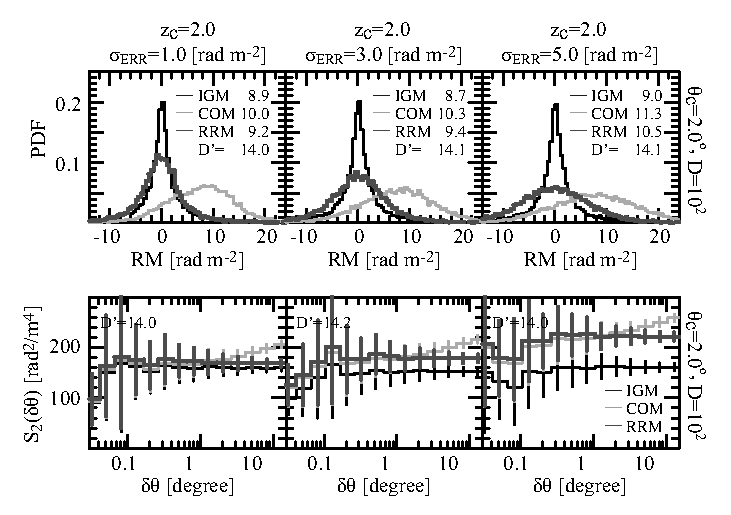
\includegraphics[width=0.7\linewidth]{magnetism/c06.s3.ss9.f1.eps}
%%%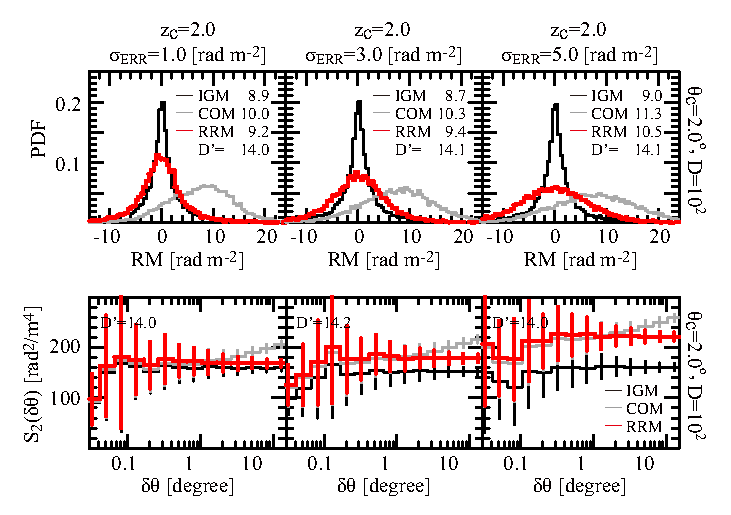
\includegraphics[width=0.7\linewidth]{magnetism/c06.s3.ss9.f1c.eps}
\end{center}
\caption{南銀極方向900平方度の模擬観測実験\citep{2014ApJ...790..123A}。採用された背景偏波源の1平方度あたりの数をD'として示してある。選ばれた偏波源について、上段はその確率密度分布、下段は2次構造関数を示す。左からランダムノイズに従う観測誤差として1, 3, 5 ${\rm rad~m^{-2}}$のRMの分散が考慮されている。細線は銀河間磁場のRMのみ、灰色線は偏波源、銀河間磁場、天の川銀河、そして観測エラーが加わった観測値、そして太線は2度のハイパスフィルターを適用した結果。介在銀河の影響のない、高赤方偏移で、そして観測誤差が小さい偏波源を選び出しハイパスフィルターをかけると、得られる結果は銀河間磁場のRMの性質をよく引き出すことができる。
}\label{c06.s3.ss9.f1}
\end{figure}

\paragraph{統計的な推定}

日本の大規模構造磁場研究の優位性として、大規模構造磁場の理論モデルに加えて、前節までに紹介してきた前景・背景の知識を豊富に有する点がある。そこで日本は、宇宙大規模構造磁場を探査する方法論の構築で世界に先駆ける。個々の視線では系外偏波源や天の川銀河の個性が強いため、銀河間磁場のRMだけを推定するのは容易ではない。そういった個性の影響を排除するのに、たくさんのデータを集めて統計的に議論することが有効である。視線上の主要な成分には平均・分散・2次構造関数などの統計に特徴があると考えられるので、その特徴から銀河間磁場のRMだけを抽出することができるかもしれない。

\paragraph{背景偏波源の観測}

前節(\S \ref{c06.s2.ss6})で紹介したとおり、膨大な数の背景偏波源から理想的なものを取り出して、銀河間磁場の寄与を推定する。SKAではそのための全天偏波源観測を提案する。それぞれの成分を考慮したRMマップのモデルを構築し、銀河間磁場のRMを推定する模擬実験が始まっている。例えば\citet{2014ApJ...790..123A}では観測されている偏波源の赤方偏移分布に従いながら、1平方度あたり100偏波源をランダムに配置し、そのうち半数が介在銀河がないものとして選び出した。そこからさらに視線に銀河団を含む偏波源ならびに赤方偏移が2以下の偏波源を除いた。そして観測誤差が小さい偏波源を選び出しハイパスフィルターをかけた。計算の結果では、ASKAP POSSUMで得られる統計(数$\mu$Jy/beamの感度で1平方度当たり100偏波源)があれば銀河間磁場RMの分散については十分な精度で推定できることがわかった(図\ref{c06.s3.ss9.f1})。SKA時代にはさらに、構造の典型的なスケールにまで示唆を得るだろう。そのためには広視野で高感度、かつ高い偏波精度の観測データを取得しなければならない。それはSKAでなければ達成できない。

\paragraph{偏波解消とトモグラフィーへの期待}

ファラデートモグラフィーは視線上の前景や背景を区別し、銀河間磁場のRMだけを抽出することができる潜在能力がある。しかし前節(\S \ref{c06.s1.ss8})で紹介したとおり、どういった観測をすれば最善かという方法論の構築が不可欠で、また合成されたファラデースペクトルを正しく解釈する経験が必要である。そこで\citet{2014PASJ...66...65A}では、ファラデートモグラフィーを使って銀河間磁場のRMを推定するための可能な方法論について詳しく議論し、実際にシンプルなモデルを使って実証を試みた。その結果、銀河系放射越しに遠方の偏波源を観測し、FDFの溝として銀河間磁場のRMを測定する方法を考案した。図\ref{c06.s3.ss9.f2}にはその概要を示す。次にシンプルなモデルを用いて実際にトモグラフィーの実証実験を行った結果、ASKAPなどの試験機世代では不定性が残るが、SKA時代には銀河間磁場のRMが10 ${\rm rad~m^{-2}}$程度以上であれば、因子2程度でFDF から直接推定できることを示した。さらに、モデルをあらかじめ仮定した観測フィット(ストークスQUデータでフィットを行うので、QU-fitと呼ばれる)では、試験機世代でも5 ${\rm rad~m^{-2}}$程度以上であれば推定できることを示した\citep{2014PASJ...66....5I}。ASKAP初期科学運用の評価やSKA1のデザイン評価のために、具体的な数値を提供している。

\begin{figure}[tbp]
\begin{center}
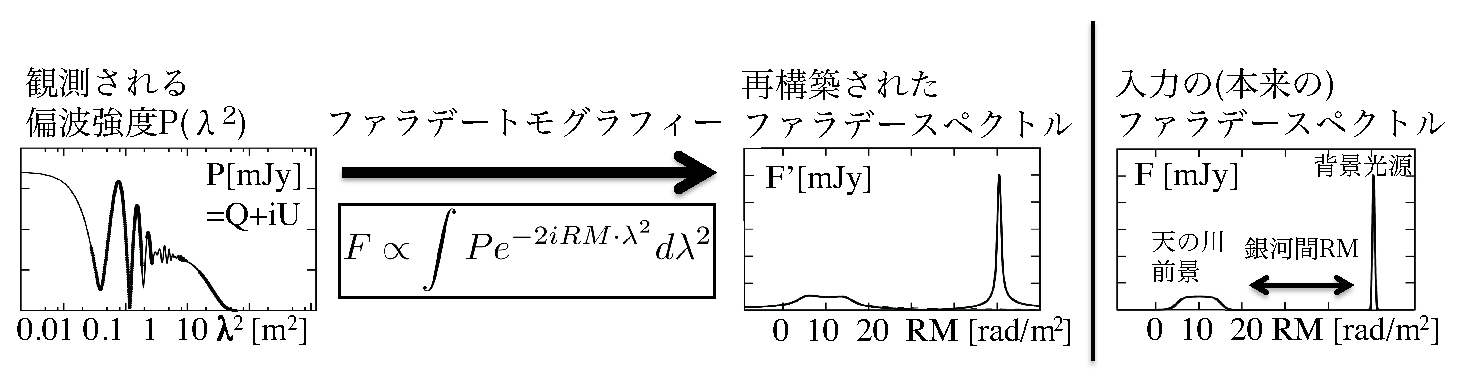
\includegraphics[width=0.9\linewidth]{magnetism/c06.s3.ss9.f2.eps}
\end{center}
\caption{ファラデートモグラフィーを活用した銀河間物質探査。\citet{2014PASJ...66...65A}を改変。
}\label{c06.s3.ss9.f2}
\end{figure}


%%%%%%%%%%%%%%%%%%%%%%%%%%%%%%%%%%%%%%%%%%%%%%%
%%%%%%%%%%%%%%%%%%%%%%%%%%%%%%%%%%%%%%%%%%%%%%%
\subsection{宇宙論的磁場生成}
\label{c06.s3.ss10}

宇宙論的磁場生成を研究する研究者は世界的にも少ないため、それ自身が日本の優位性といえるだろう。日本における宇宙論的磁場に関する研究は、前節までの議論にあったように、初期宇宙、特に晴れ上がり期や初代星形成期での磁場生成に関して世界をリードしている。従って日本の宇宙磁場科学検討班では、引き続きこの研究分野で世界に先駆けた成果をあげていくことを目指す。以下ではその例として、班内で研究が進展している密度揺らぎおよびtopological defectによる磁場生成などを議論する。

\paragraph{晴れ上がり期の2次オーダーの密度揺らぎ}

晴れ上がり期以前のプラズマ宇宙では、光子とバリオン流体の速度差および光子の非等方圧力が磁場の源になることが明らかになっている\citep{2006Sci...311..827I}。宇宙大規模構造の種になる密度揺らぎからは、線形理論の範囲では磁場は生成されないが、高次の効果で磁場が生成される。\cite{Saga.et.al.2015}はこれまでの計算を拡張し、高次の効果をすべて取り入れた計算に成功しつつある。密度揺らぎの統計的性質(強度や相関など)は、CMBの精密観測により既知であるので、ここで計算された磁場は宇宙に必ず存在する磁場の初期条件を与えるものとして重要である。準備中の結果を図\ref{c06.s3.ss10.f1}左に示す。スペクトルからは小スケールほど磁場が大きく生成されることが分かる。これは磁場の観測を通じて、CMBの観測では到達できない小スケールの密度揺らぎへの制限が可能であることを示唆している。

\paragraph{晴れ上がり期の位相欠陥}

大統一理論(GUT)などの力の統一理論では多くのスカラー場の存在が示唆されている。これらが宇宙の温度の低下とともに相転移を起こすことで、様々な種類の位相欠陥(topological defect)が宇宙に存在する可能性がある。これら位相欠陥は密度揺らぎ、重力波とともに宇宙に回転型の揺らぎを励起するため、磁場の源となり得る。\cite{Horiguchi.et.al.2015}は位相欠陥の一つの型であるテクスチャーについて、上記の機構によって生成される磁場の大きさを計算している。準備中の結果を図\ref{c06.s3.ss10.f1}右に示す。位相欠陥の存在を示す観測的な証拠は未だないが、この結果は$10$ kpcというスケール、赤方偏移$z \sim 10$で$\sim 10^{-18}$ Gという大きさの磁場が生成されうる可能性を示しており、これはのちに議論するように将来の観測によって検証可能かもしれない。宇宙論的磁場の観測が初期宇宙の新しいプローブとして用いられるように、テクスチャー以外にも、宇宙ひもやモノポール等に関しても検討を進める必要がある。

\begin{figure}[tbp]
\begin{minipage}[c]{0.5\textwidth}
\centering
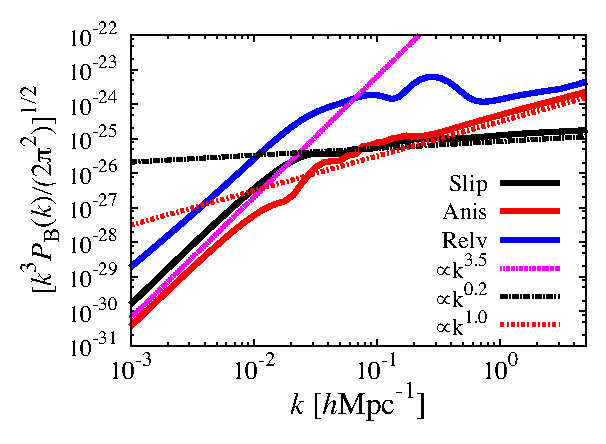
\includegraphics[width=\linewidth]{magnetism/c06.s3.ss10.f1a.eps} 
\end{minipage}
\begin{minipage}[c]{0.5\textwidth}
\centering
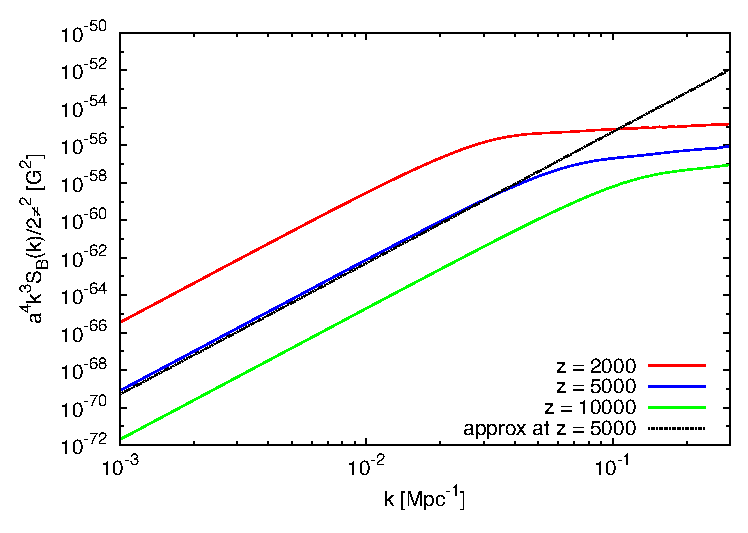
\includegraphics[width=\linewidth]{magnetism/c06.s3.ss10.f1b.eps} 
\end{minipage}
\caption{宇宙の晴れ上がり期に生成される磁場のパワースペクトル。左図は密度揺らぎ起源、右図はテクスチャーと呼ばれる位相欠陥起源のものである。
}\label{c06.s3.ss10.f1}
\begin{center}
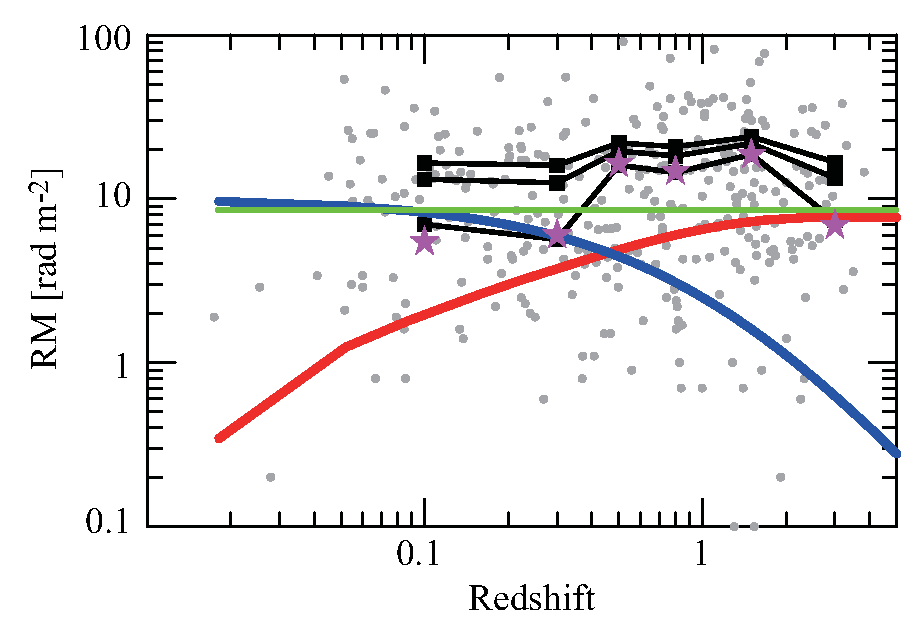
\includegraphics[width=0.8\linewidth]{magnetism/c06.s3.ss11.f1.eps}
\end{center}
\caption{赤方偏移とRMの関係。灰色点は銀緯$|b|> 75^\circ$の317のRM観測値\citep{1209.1438v2}、黒は観測誤差0, 10, 15 ${\rm rad~m^{-2}}$を仮定して観測値から差し引いた$z=0-0.2$ (71点), $0.2-0.4$ (50), 0.4-0.6 (31), 0.6-1.0 (55), 1.0-2.0 (77)のRMの分散。青は$z=0$で10 ${\rm rad~m^{-2}}$を仮定した偏波源のRMの分散の期待値。赤と緑は銀河間磁場\citep{2011ApJ...738..134A}と天の川銀河\citep{2010MNRAS.409L..99S}のRMの分散の期待値。紫は観測値から緑・青・赤を差し引いた残差として予想される介在銀河のRM(観測誤差は12.5 ${\rm rad~m^{-2}}$を仮定)。
}\label{c06.s3.ss11.f1}
\end{figure}

\paragraph{天体形成時での磁場生成}

通常、初代天体形成時にはダイナミクスに影響を与えるほど強い磁場が存在することはないと考えられることが多い。ところが、最近になってダークマターが重力崩壊しミニハローが形成された際に自然に磁場が生成され、その後乱流によってダイナミクスに影響を与える強さにまで磁場が増幅されているのではないかということが指摘されている\citep{2008ApJ...688L..57X,2010ApJ...721L.134S}。天体形成は、重力崩壊したミニハローの中のガスがさらに収縮して起こると考えられているため、宇宙最初の天体形成時においても磁場の存在を無視できないかもしれない。例えば初代天体の初期質量関数は、宇宙再電離の歴史を決める重要な要素であるため、磁場の存在がどれほどの影響を初代天体形成へ与えるかを調べることは重要であろう。

\paragraph{偏波解消とトモグラフィーへの期待}

上記の磁場生成研究において明らかになっていることは、生成される磁場の強度がとても小さいことである。従って、現在の宇宙においてこれらの宇宙論的な磁場を観測するためには、少なくともその後の天体形成による磁場の``汚染"が比較的進んでいない銀河間及びボイド領域で観測する必要がある。ファラデートモグラフィーでは、放射の少ない銀河間およびボイド領域での磁場のシグナルはファラデースペクトルでのギャップとして現れる。今後は宇宙論的体積の大規模シミュレーションなどを行い、SKA時代での銀河間、ボイド磁場の検出限界などを調べる予備研究が重要であろう。一方、再電離期以前の高赤方偏移時代は天体形成による磁場の汚染が比較的少なく、宇宙論的磁場の観測ターゲットと考えられる。最近、ファラデートモグラフィーとは別に、SKA時代での磁場の検出法について興味深い手法が提案された\citep{1410.2250}。それによると、再電離期での宇宙論的磁場の存在が、宇宙論的21cm線シグナルの統計的等方性を破り、その観測によって赤方偏移$z\gtrsim 10$程度で$10^{-19}$Gの磁場の検出が可能となると主張している。この方法による磁場の観測可能性については宇宙再電離についての専門家と協力して研究を進めて行くのが重要だろう。


%%%%%%%%%%%%%%%%%%%%%%%%%%%%%%%%%%%%%%%%%%%%%%%
%%%%%%%%%%%%%%%%%%%%%%%%%%%%%%%%%%%%%%%%%%%%%%%
\subsection{宇宙磁場の宇宙論的進化}
\label{c06.s3.ss11}

\paragraph{RMと赤方偏移}

日本のサイエンスの最後のひとつとして、RMと赤方偏移の関係を取り上げる。HI観測や可視光観測とのクロスIDによって系外偏波源の赤方偏移が分かれば、その赤方偏移と系外偏波源のRMとの関係をプロットすることができる。それは磁場の宇宙論的進化を理解するための最も分かりやすい手段といえるだろう。これまでにもRMのサーベイデータが得られるたびに、その関係を発見しようとする試みがなされてきた。しかし、前節で最新の結果を紹介している通り\citep{1209.1438v2,1405.5087}、観測の誤差の不定性が大きく、データの選択による恣意的な結果も排除しきれていない。国内でも科学検討班が結成当初から継続して調査を進めているが、不定性に悩まされている。

\paragraph{成分ごとの進化史}

系外偏波源のRMと赤方偏移との関係をプロットした図には、系外偏波源の磁場、銀河間の磁場、介在銀河の磁場、天の川銀河の磁場、そして観測誤差などの影響が混在しうる。一つ例を示す。図\ref{c06.s3.ss11.f1}には、高銀緯方向に位置する系外偏波源のRMを赤方偏移の関数としてプロットした\citep{2014ApJ...790..123A}。まず、天の川銀河の寄与だけが銀緯と相関する性質から、高銀緯方向の天の川銀河RMの分散の期待値は8.4 ${\rm rad~m^{-2}}$と見積もられている\citep{2010MNRAS.409L..99S}。近傍($z=0-0.2$)の系外偏波源のRMの分散はその値を上回っており、系外からの寄与が期待される。ここで、近傍の場合視線距離が比較的短いため、介在銀河や銀河間磁場の寄与は小さい。故にこの系外からの寄与の大半は偏波源と考えられるので、その統計的な寄与は10 ${\rm rad~m^{-2}}$程度である。次に高赤方偏移に向かうと、偏波源のRMは$(1+z)^2$の赤方偏移の影響を受ける。もし偏波源の密度や磁場が赤方偏移の関数として変化しなければ、図の青線のように偏波源のRMの観測値への寄与は減少していく。一方で銀河間磁場の寄与は視線距離が伸びることで赤線のように増加していくだろう\citep{2011ApJ...738..134A}。これらに加えて、一部の偏波源の前景には介在銀河が存在し、RMに少なからず寄与しているかもしれない。

\paragraph{背景偏波源の観測}

これまでに説明されてきた通り、この研究でも膨大な数の背景偏波源を得るため、全天あるいは銀極方向の深い偏波源観測を提案する。それはSKAでなければ達成できない。

\paragraph{偏波解消とトモグラフィーへの期待}

偏波解消とファラデートモグラフィーを用いて、初めて上記の方法論の適用を本格化できる。それぞれの成分の進化史を分けて議論することが可能になる。


%%%%%%%%%%%%%%%%%%%%%%%%%%%%%%%%%%%%%%%%%%%%%%%
%%%%%%%%%%%%%%%%%%%%%%%%%%%%%%%%%%%%%%%%%%%%%%%
\subsection{トモグラフィーの諸問題の改善}
\label{c06.s3.ss12}

\paragraph{トモグラフィーのコード開発実績}

科学検討班ではファラデートモグラフィーのソフトウェア開発を進めてきており、特にQU-fittingと呼ばれるモデルフィット法のソフトウェアをASKAPの偏波サーベイ計画であるPOSSUMのデータパイプラインへ導入している。このソフトウェアではファラデースペクトルを複数のガウス関数からなるものと仮定して、その個数や幅、中心のファラデー深度、偏波角などをパラメータとしている。そしてマルコフ連鎖モンテカルロ法(MCMC)によって観測データをフィットすることによって、ガウス関数の個数を情報量規準(AICやBIC)を用いて決定し、その他のパラメータの信頼区間を得る。MCMCは天文学において近年よく用いられるデータ解析法であり、モデルのパラメータ数が多くても計算量があまり増えない効率的な方法である。しかし単純なメトロポリス法では、パラメータ空間における尤度の構造が複雑であると収束が遅かったり最大尤度のパラメータ値に到達しないなどの問題がある。SKAにおいてはトモグラフィーを適用する天体数は膨大なので、計算量の問題は深刻である。また、ガウス関数の個数を選ぶための情報量規準は尤度の分布がガウス関数であるとの仮定や、観測データが無限にあるとした仮定に基づく近似的なものであり、その有効性には注意が必要である。

\paragraph{レプリカ交換モンテカルロ法}

これらの問題を解決する方法として、我々はレプリカ交換モンテカルロ法という手法を導入することを目指している。これはパラメータ空間における尤度の構造を滑らかにするための「温度」を導入し、複数の温度で観測データのフィットを行うことによって最大尤度となるパラメータ値への収束を高速化するものである。また計算過程で得られる自由エネルギーはAICやBICよりも適用範囲の広い情報量規準になり、ガウス関数の個数の決定もより正確に行うことができると期待される。この方法によって1天体あたり1分程度の時間でモデルフィットを行うソフトウェアを構築することを目指す。

\paragraph{使用するモデルの関数形}

また、使用するモデルの関数形をどう決めるかというモデルフィット法の原理的な問題にも取り組む。銀河や銀河団などのモデルからファラデースペクトルを計算し、現実にはファラデースペクトルがどういう形をしているのか、どういう特徴を引き出すことが重要なのかを検討することによってモデルフィットに用いる関数形を決める。

\paragraph{RM CLEANの応用}

最後に、マルコフ連鎖の初期条件としてRM CLEANの結果を使うオプションを検討する。RM CLEANによって偏波源の数を推定し、その幅やファラデー深度などの推測値を連鎖の初期条件に使うことによってより収束が速くなることが期待される。しかしこれはそもそもRM CLEANが正しい推定値を与えなければ意味がない。\cite{2014PASJ...66...61K}で明らかにされたように単純なRM CLEANにはファラデー深度が近い2つの源があると偽の源が出現してしまうという欠陥がある。圧縮サンプリングの手法などを応用してより信頼できるRM CLEANアルゴリズムを開発し、マルコフ連鎖の初期条件としての応用を目指す。


%%%%%%%%%%%%%%%%%%%%%%%%%%%%%%%%%%%%%%%%%%%%%%%
%%%%%%%%%%%%%%%%%%%%%%%%%%%%%%%%%%%%%%%%%%%%%%%
\subsection{さらなるシナジーを求めて}
\label{c06.s3.ss13}

\paragraph{太陽・恒星の偏波解析による磁場の導出}

日本のサイエンスの優位性として、日本における太陽研究からの知見を欠かすことはできない。太陽から放出される電波は、放射源の磁場の影響で円偏波成分を持つことが知られている。近年、センチ波の電波干渉計である野辺山電波ヘリオグラフを用いた偏波観測から、熱制動放射による円偏波、磁気共鳴放射による円偏波、モードカップリングによる円偏波の反転現象などを利用して、太陽大気の磁場を導出する試みがなされてきた\citep{2013PASJ...65S..14I}。太陽において電波の発生周波数は発生領域の高度におおよそ対応する。よって広帯域に偏波の撮像観測ができれば、太陽コロナの3次元的な磁場構造及びその時間変動が導出でき、太陽コロナの様々な電磁流体現象(フレアやコロナ質量放出現象など)と磁場の関係が観測的に明らかにできる。更に、高分解能かつ高感度な性能があれば、太陽以外の恒星で磁場を導出できる可能性がある。日本には、メートル波からセンチ波にかけての単面鏡の太陽電波望遠鏡も複数存在する。これらの太陽電波望遠鏡群から得られるデータを組み合わせると、SKAの全観測周波数において偏波スペクトルデータが得られる。単面鏡によるスペクトル観測では、ビームサイズが太陽の視直径より大きくなるよう設定し、太陽全面から来る電波放射を受信できるようにする。これは空間分解能が無いことを意味するが、一方で、デジタルバックエンドを工夫することで、10ms以下の高時間、60kHz以下の高周波数分解観測を達成し、ユニークな科学成果を出せる。これはSKAと同じ周波数帯域で相補的な観測方式と言え、今後SKAと協力することで、日本独自のサイエンスを提案できると期待される。

\paragraph{最高エネルギー宇宙線の磁場による偏向の解明}

\begin{figure}[tbp]
\begin{center}
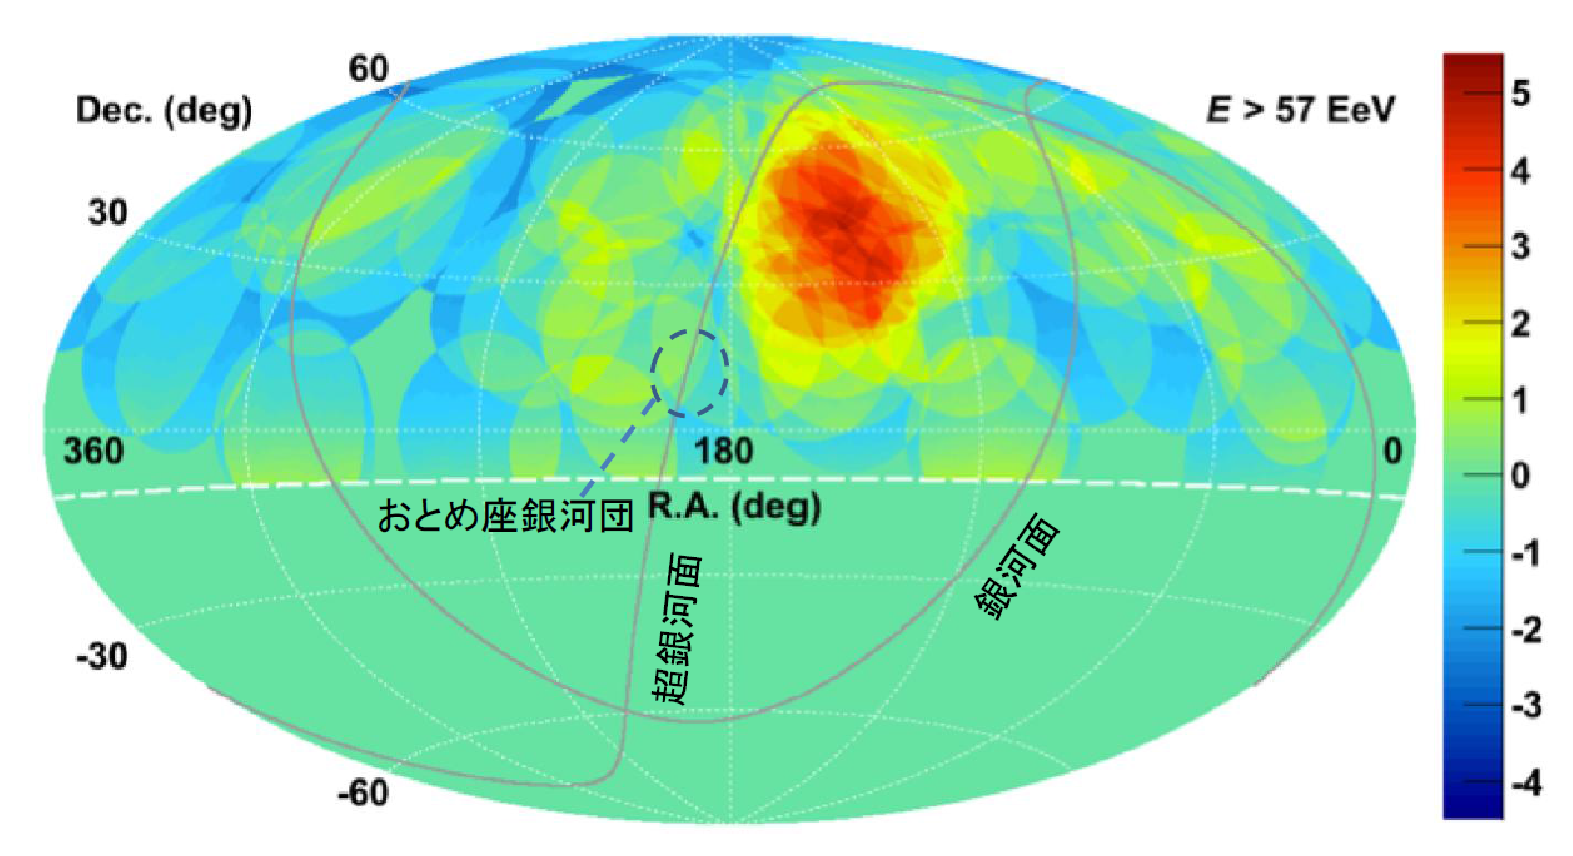
\includegraphics[width=0.8\linewidth]{magnetism/c06.s3.ss13.f1.eps}
\end{center}
\caption{TA実験5年間の観測から得られた5.7$\times 10^{19}$ eV以上の最高エネルギー宇宙線72イベントの有意度マップを赤道座標で示した。有意度は、それぞれの宇宙線の到来方向から半径20度の領域を重複して数えたイベント数の分布の、等方分布からのずれを評価している。一番濃い赤い色(赤軽146.7$^{\circ}$、赤緯43.2$^{\circ}$)を中心とした半径20度の円の中に、19イベントが観測され、一様な到来分布の場合の期待数は4.5イベントである。
}\label{c06.s3.ss13.f1}
\end{figure}

日本のサイエンスの優位性として、日本のグループが参画するテレスコープアレイ実験(TA実験)との協力も重要である。TA実験は、米国ユタ州に約700 km$^2$の面積を覆う1.2 km間隔に配置された507台の地表粒子検出器(SD)アレイと、それを囲む3つの大気蛍光望遠鏡(FD)ステーションの2種類の検出器の両方を用いて、2008年5月から超高エネルギー宇宙線の観測を行っている。宇宙線は宇宙を飛び交う高エネルギーの陽子や原子核であり、地球への宇宙線の到達頻度は$10^{10}$電子ボルト(eV)から$10^{20}$ eVまで10桁以上にわたってエネルギーのほぼ3乗のべき関数で減少している。$10^{19}$ eVくらいまでは一様等方に地球に飛来しており、確認されている異方性は0.1\%に過ぎない。TA実験では、5年間のSD観測から得られた5.7$\times 10^{19}$ eV以上の72イベントを解析した結果、到来する方向が特定の領域に集中(約400\%の異方性に相当)するホットスポットの兆候を約3.4$\sigma$ (99.963 \%)の有意度で検出した\citep{2014ApJ...790L..21A}。図\ref{c06.s3.ss13.f1}は72イベントの宇宙線の到来方向から得られた有意度のマップである。FDの観測結果によると、$10^{18.2}$ eV以上のエネルギーの宇宙線は軽元素で、陽子が主と考えられる。異方性の検出された5.7$\times 10^{19}$ eV以上の宇宙線を放出する宇宙線源は、GZK効果などで知られる宇宙背景放射の光子との相互作用によるエネルギー損失のため、約250 Mpc以内の近傍に限られる。このような近傍の宇宙の質量の分布は超銀河面やおとめ座銀河団に集中しているが、最も有意度の高い方向は超銀河面からは19度離れており、おとめ座銀河団からは更に離れている。また、その方向には際立った天体はこれまで見つかっていない。このことは約250 Mpc以内の磁場(天の川銀河や大規模構造)による宇宙線の偏向を示唆する。SKAでファラデートモグラフィーの方法を用いれば、それぞれ磁場の成分を分離して観測できる可能性があるので、磁場による偏向、更には最高エネルギー宇宙線の起源解明への手がかりを与えると期待される。

\paragraph{再電離21cm線前景放射の除去}

ファラデートモグラフィーの新たな応用例として、宇宙再電離期の中性水素からの21cm線放射の観測における前景除去についても検討していく。再電離期の21cm線シグナルのパワースペクトルは銀河系放射や系外電波天体などの前景放射に比べて$10^{-6}$ほどの大きさであり、前景放射の除去が大きな課題になっている。最近、LOFARグループによって偏波に関する前景放射の除去も重要であることがわかってきており、銀河系のシンクロトロン放射による偏波強度を高精度に較正する必要が指摘されている。我々は再電離グループとの協働のもと、上記のソフトウェアを応用してこの問題に取り組む予定である。

\paragraph{宇宙マイクロ波背景放射}

宇宙マイクロ波背景放射(CMB)の研究は、紛れもなく宇宙磁場研究のひとつである。天の川銀河や大規模構造の磁場・放射がCMB研究に与える影響は重要な研究課題である。また、CMBを偏波源として使うアイデアが日本から提案されている\citep{2003ApJ...584..599O}。現状では技術的に困難ではあるが、実現すれば強力なツールとなるだろう。





